\chapter{Eye information}
This chapter provides an introduction to eye-tracking systems and their uses as well as what constitutes sensitive information in eye tracking. 

I define an \gls{eye-system} as a system which attempts decoding of human properties through use of human eye images. Any such system must overcome 

\todo{figure out}
This chapter provides an overview of an \gls{eye-system}. I define an eye information process as any process that uses a human eye as its input and has the aim of extracting some property of interest from it. The term thus covers both systems that analyse eye movement, i.e. eye-tracking, and eye appearance, e.g. iris recognition, retinal imagery, etc. 


The model is based on a general idea of \gls{eye-system}s. This is the kind of system introduced in \cref{sec:eye-tracking} but should be understood in a more general manner

The first section provides an overview of the anatomy of human eyes. It serves as a reference for easily understanding how eye information processes uses the anatomy for their operation as well as what the physical limitations are. 

Next, the foundations of modern eye-tracking systems will be presented. The goal is to provide the reader with a birds-eye view of the field and its methods.

The final section focuses on sensitive information. Both appearance-based extraction techniques such as iris recognition and gaze-based techniques such as attention-analysis will be presented. 


\section{Anatomy}
Our eyes are an essential part of the human existence. What is so special about the eyes is that they are not just sensory apparatuses for enabling us to register many properties of the physical world around us but also reveal a wealth of information about their owner's current physical and mental state. From a social perspective, eye movements communicate where their owner are looking which typically corresponds with their focus of attention. Additionally, eyes are clearly used socially as indicators of well-being as well as social interaction, i.e. by looking into the eyes of other people. It is likely no coincidence that the eyes have often mythologically been described as doorways to the soul or in some other way been seen as a logical end-point of our minds. To see is often analogous to understand or realise. 

\begin{figure}
    \centering
    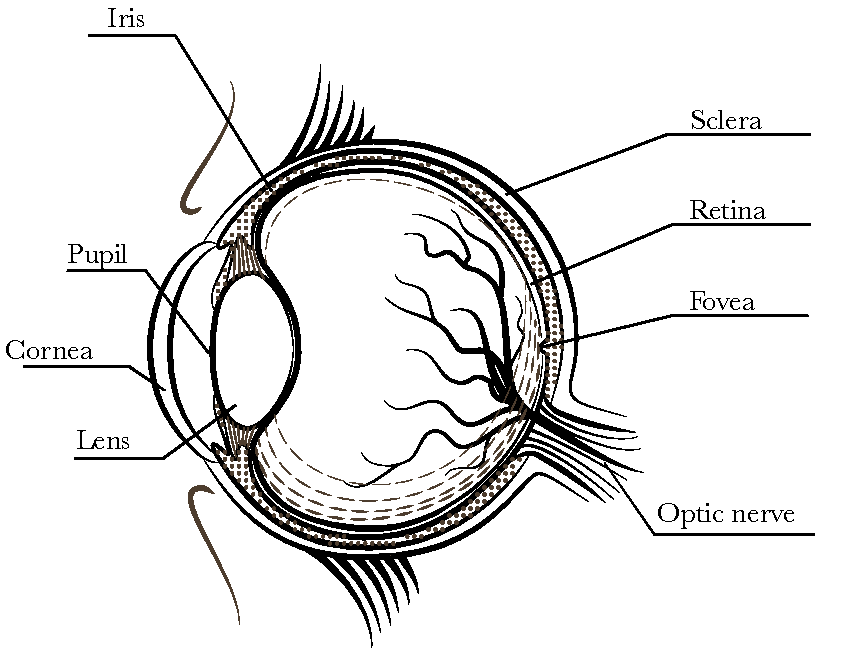
\includegraphics[width=0.8\linewidth]{figures/eye.pdf}
    \caption{Diagram of the human eye. A number of significant features have been marked. Image adapted in accordance with licence from \cite{freepik}.}
    \label{fig:anatomy}
\end{figure}

From a physiological perspective, the eye is an incredibly complex organ which reacts in variou...


\Cref{fig:anatomy} shows an overview of a human eye. It is shaped approximately like a sphere with a bulge where the \emph{cornea} is places. The most interesting areas from the perspective of eye information processes, are the retina and the frontal lens complex. 

\todo{remember references}
The \emph{retina} is a tissue covering the inside of the eye. It is composed of light sensitive neurons called photoreceptors, which react to either a wide (rods) or narrow (cones) band of light bandwidths. The rods are used for black/white vision, typically in low-light conditions due to their much higher sensitivity than cones. Cones are primarily used for colour vision as there are three types which each respond to a specific band of wavelengths. Cones have a much higher concentration around a small area on the retina called the \emph{fovea}. This area enables high visual acuity and is therefore generally considered the primary place of attention. In fact, it is well-known that, in spite of the rapid drop-off in photoreceptor density outside the fovea, the human brain succeeds in combining visual information from many individual fixations to produce what seems like high-resolution visual perception.

\begin{figure}
    \centering
    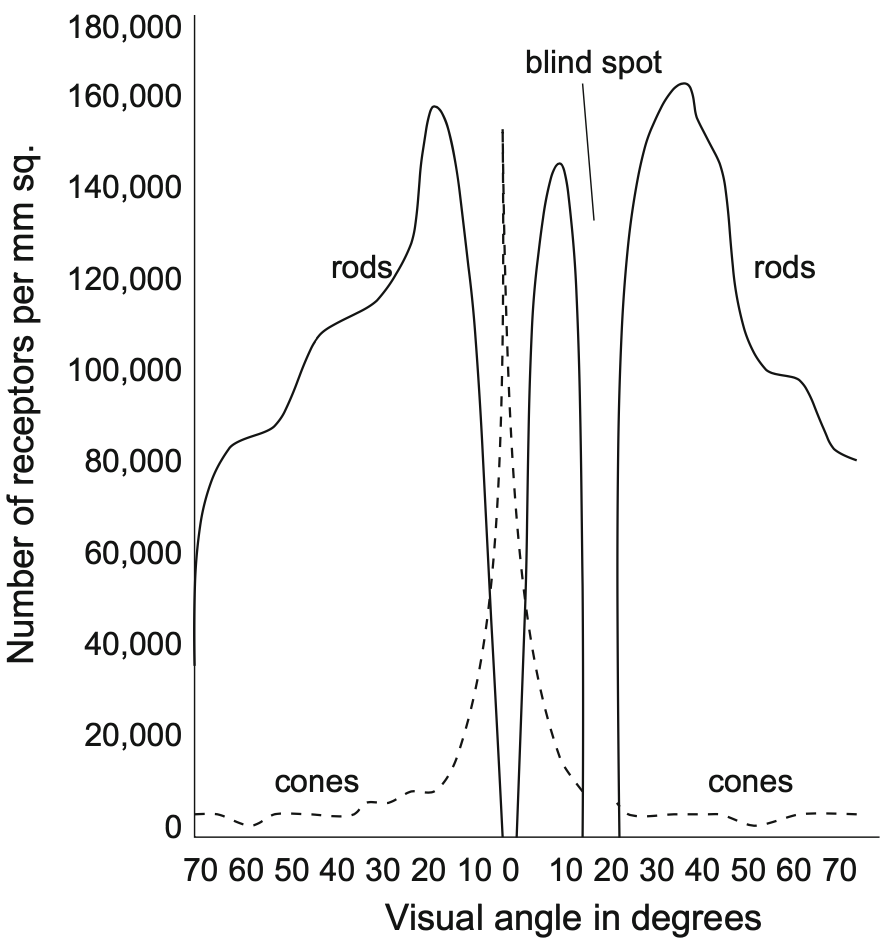
\includegraphics[width=0.6\linewidth]{figures/retina-density.png}
    \caption{Photoreceptor density as a function of visual angle (centred at the fovea). From \parencite{methodology}.}
    \label{fig:my_label}
\end{figure}

The fovea is very important for determining gaze direction or point-of-regard since it determines what is known as the \emph{visual} axis which intersects the lens centre and fovea. This visual axis typically varies slightly (about 5 degrees) from the \emph{optical axis} which intersects the cornea, pupil, and lens. This variation is different from person to person which has to be corrected by an eye-tracker. Typical modern eye-trackers have gaze direction errors of about $0.5^\circ-1.5^\circ$ which is much lower than the $\pm 5^\circ$ of the visual axis.

The frontal lens complex contains the components that allow light to enter the eye in a controlled manner. The lens system is composed of the static \emph{cornea} which accounts for a majority of the eye's optical power and the \emph{lens} which is adjusted by muscles called \emph{ciliary bodies} located behind the iris. The \emph{iris} is composed of muscles that control the size of the circular opening in its middle known as the \emph{pupil}. This allows the eye to adjust the amount of light entering the eye. 

\subsection{Eye movements}
Eye movements are formed of both conscious, semiconscious, and unconscious actions. This has led to great interest in studying these movements for various purposes, including behavioural studies as well as ...

There are five basic categories of eye movements: saccades, vergence movements, smooth pursuits, vestibular, and physiological nystagmus \parencite[39]{methodology}. Saccades are further subdivided into macro- and micro-saccades. Macro-saccades are the typical jerky movements we perform when moving from fixation to fixation. Micro-saccades are involuntary movements of $0.03-2$ degrees. The purpose of micro-saccades is to change the light-stimulus on the retina, since continuous stimulus of photoreceptors results in decreasing activation strength over time \parencite[44]{methodology}. Smooth pursuits are a mode of movement where the eye follows a fixation point on a moving object. Vergence movements are relative movements of the left and right eye to ensure vergence of the visual axes at the point of fixation \parencite{methodology}.


\section{Eye-tracking}\label{sec:eye-tracking}
\Gls{eye-tracking} covers the processes of detecting the location and movements of eyes and estimating \gls{gaze}. Gaze is defined as either a specific \acrfull{por} or as a \emph{direction}. Today, this is done exclusively through image based techniques (REF) but intrusive methods, typically using some form of special contact lens in combination with a sensor, also exist (REF).

\subsection{Why}
\begin{figure}
	\centering
	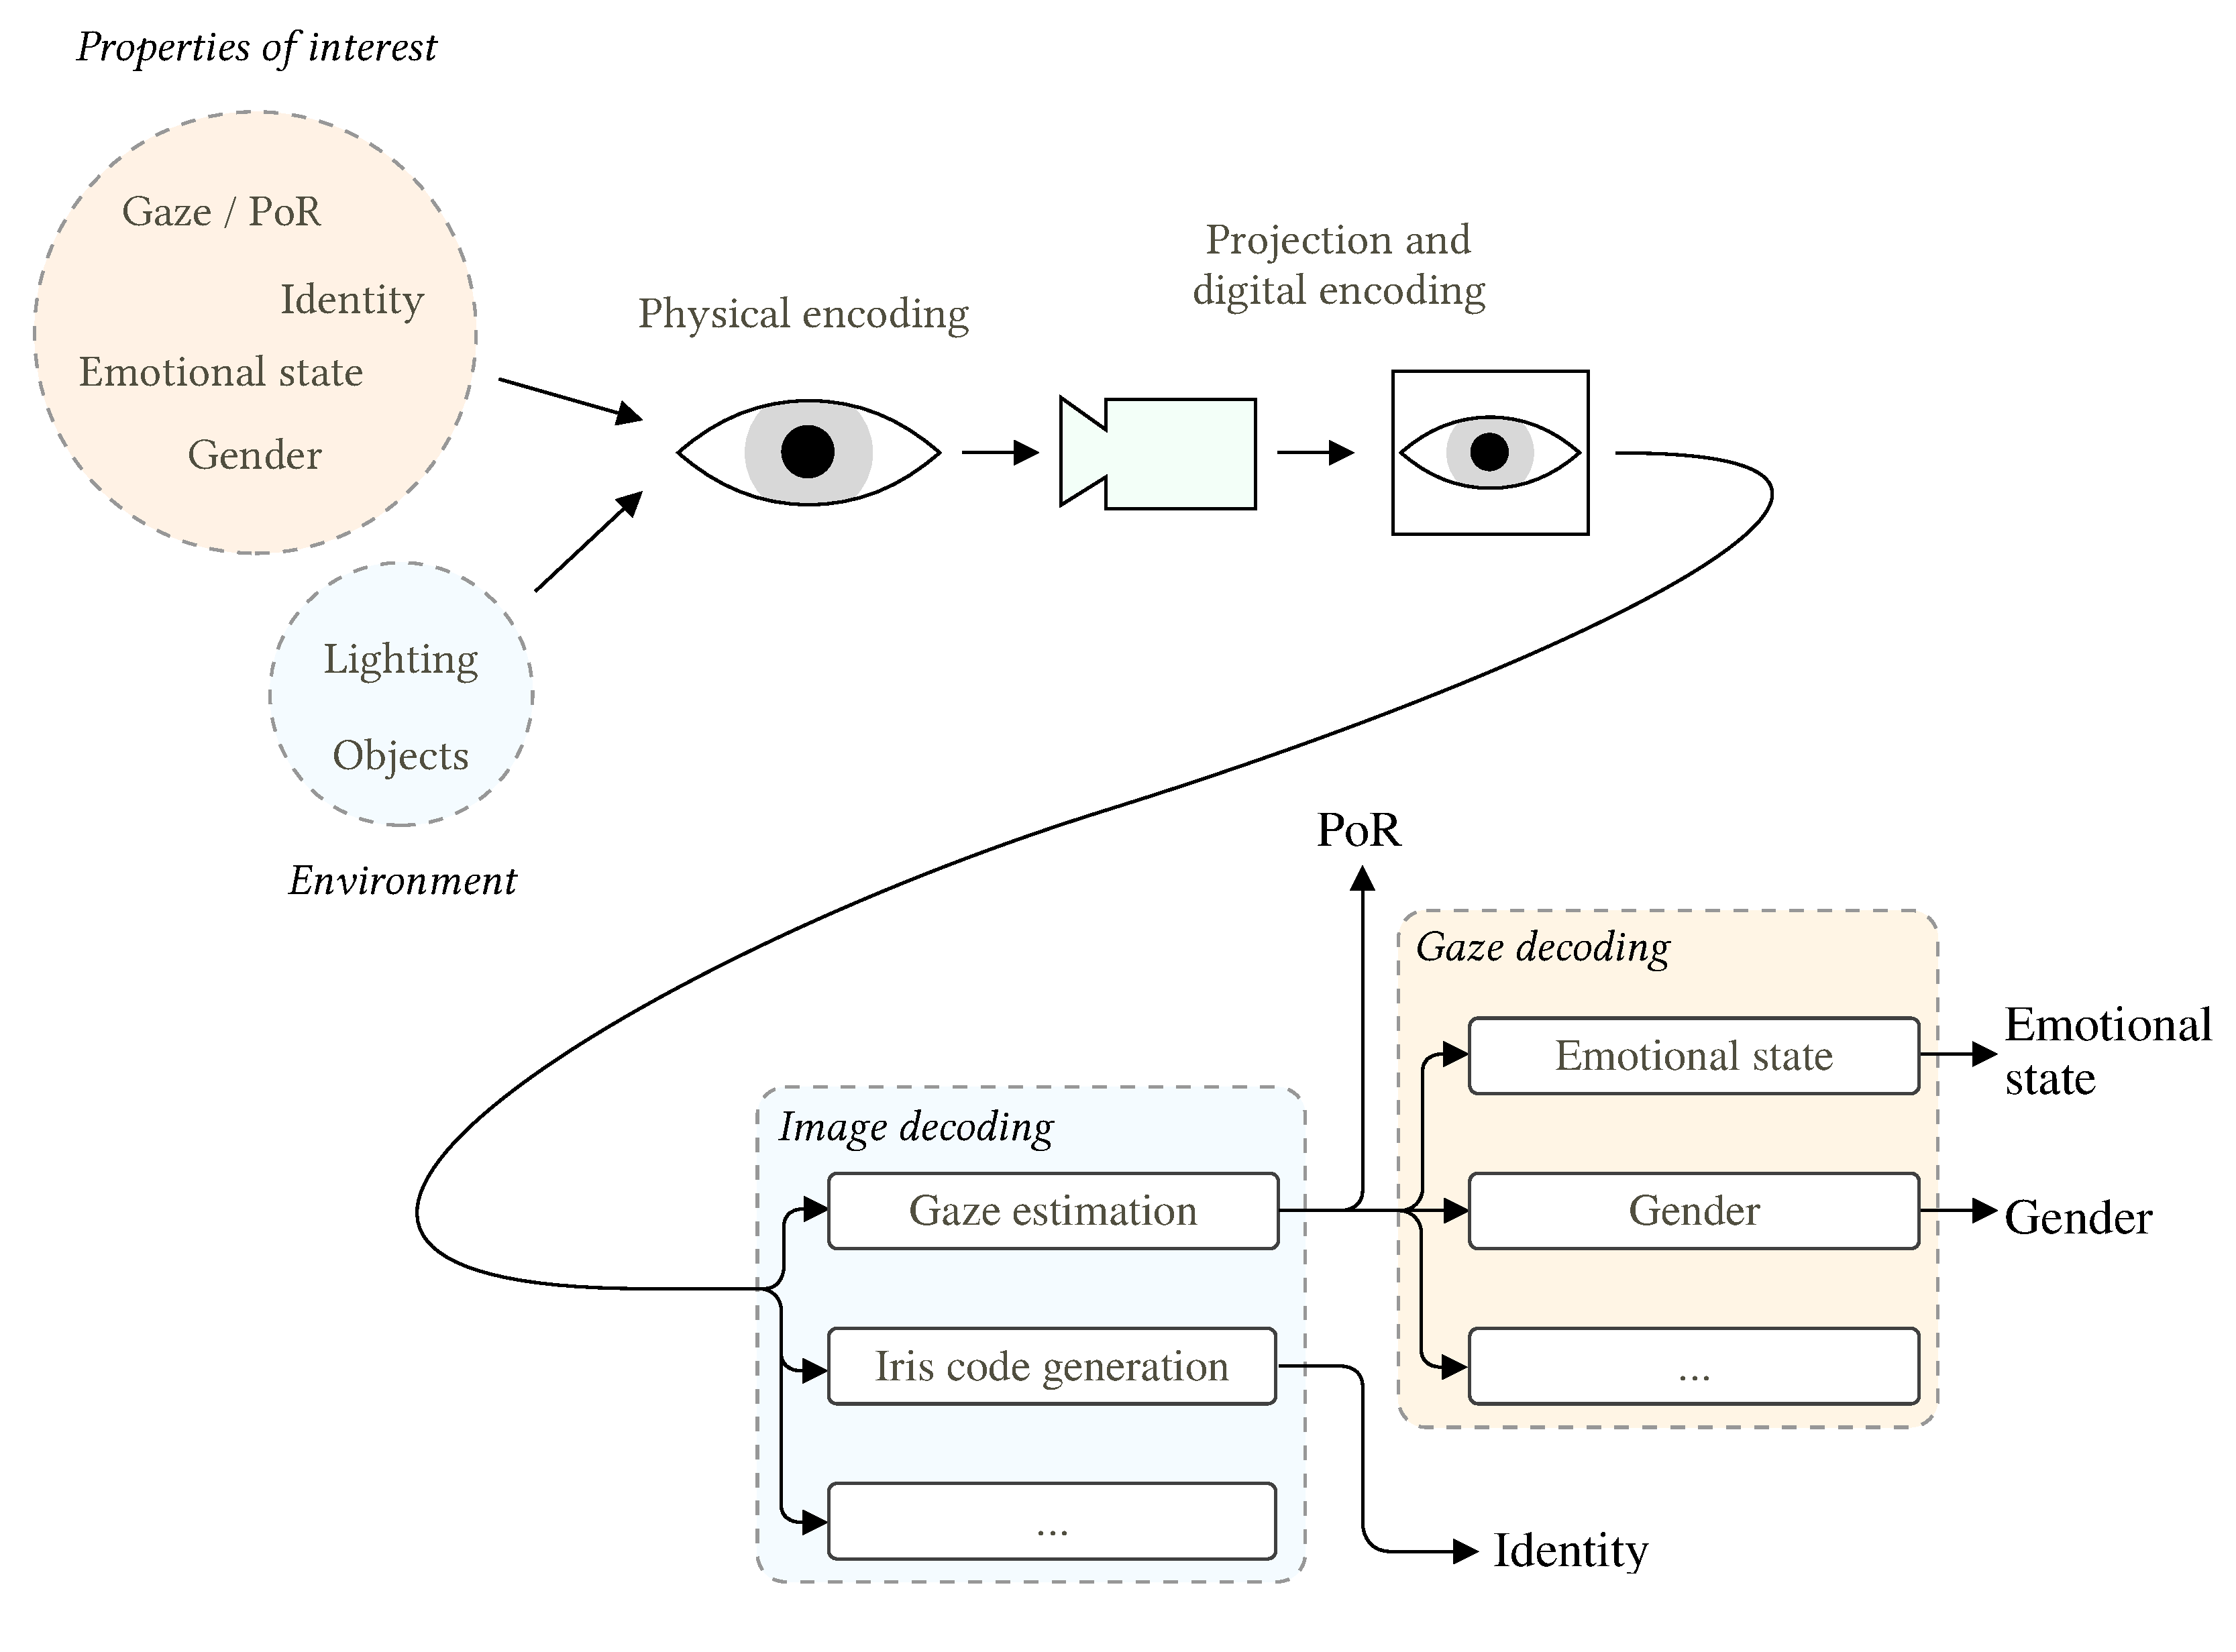
\includegraphics[width=1\textwidth]{figures/model/eye-tracking-model}
	\caption{Model overview}\label{fig:eye-tracking-model}
\end{figure}

\Cref{fig:eye-tracking-model} shows a graphical overview of an eye information processing system (EIPS). It is functionally \todo{finish this}



To understand \gls{eye-tracking}, we first need to understand the purposes for which it was made. \todo{finish}

In terms of research, \gls{eye-tracking} has traditionally been of interest in psychology (REfs) and physiology (REFS) studies due to the close connection between gaze and attention and the prominent use of eyes in humans everyday lives. A typical application is the study of visual attention, i.e. where a person is looking in a specific situation over time. Examples include studies of driver behaviour (REF), shopping behaviour (REF), analysis of reading ability and how reading works (REF), how the eyes are used in elite sports and whether analysis may be used for athletic improvements (REFS), and many more. In the medical industry, eye-tracking has been used as a tool in diagnosis of both psychological and physical conditions (REF). 

Most importantly for this thesis however, are applications in \acrfull{hci} which is a term that covers technologies or systems that act as interfaces between humans and computers (REF). The rapid decrease in part costs has made consumer-level and large-scale medical \acrlong{hci} feasible. Major corporations investing in \acrfull{vr} technologies including NVidia and Facebook, have started major research efforts towards enabling low-cost and precise eye-tracking built into \acrshort{vr}-headsets (REF). In the medical industry, technologies such as tablets have already been deployed on large scales to enrich the communication abilities of people suffering from various diseases (REF). Eye-tracking technologies that are easier to use and simpler to set up are actively being researched as well (REF). 

\subsection{How it works}
\begin{figure}
	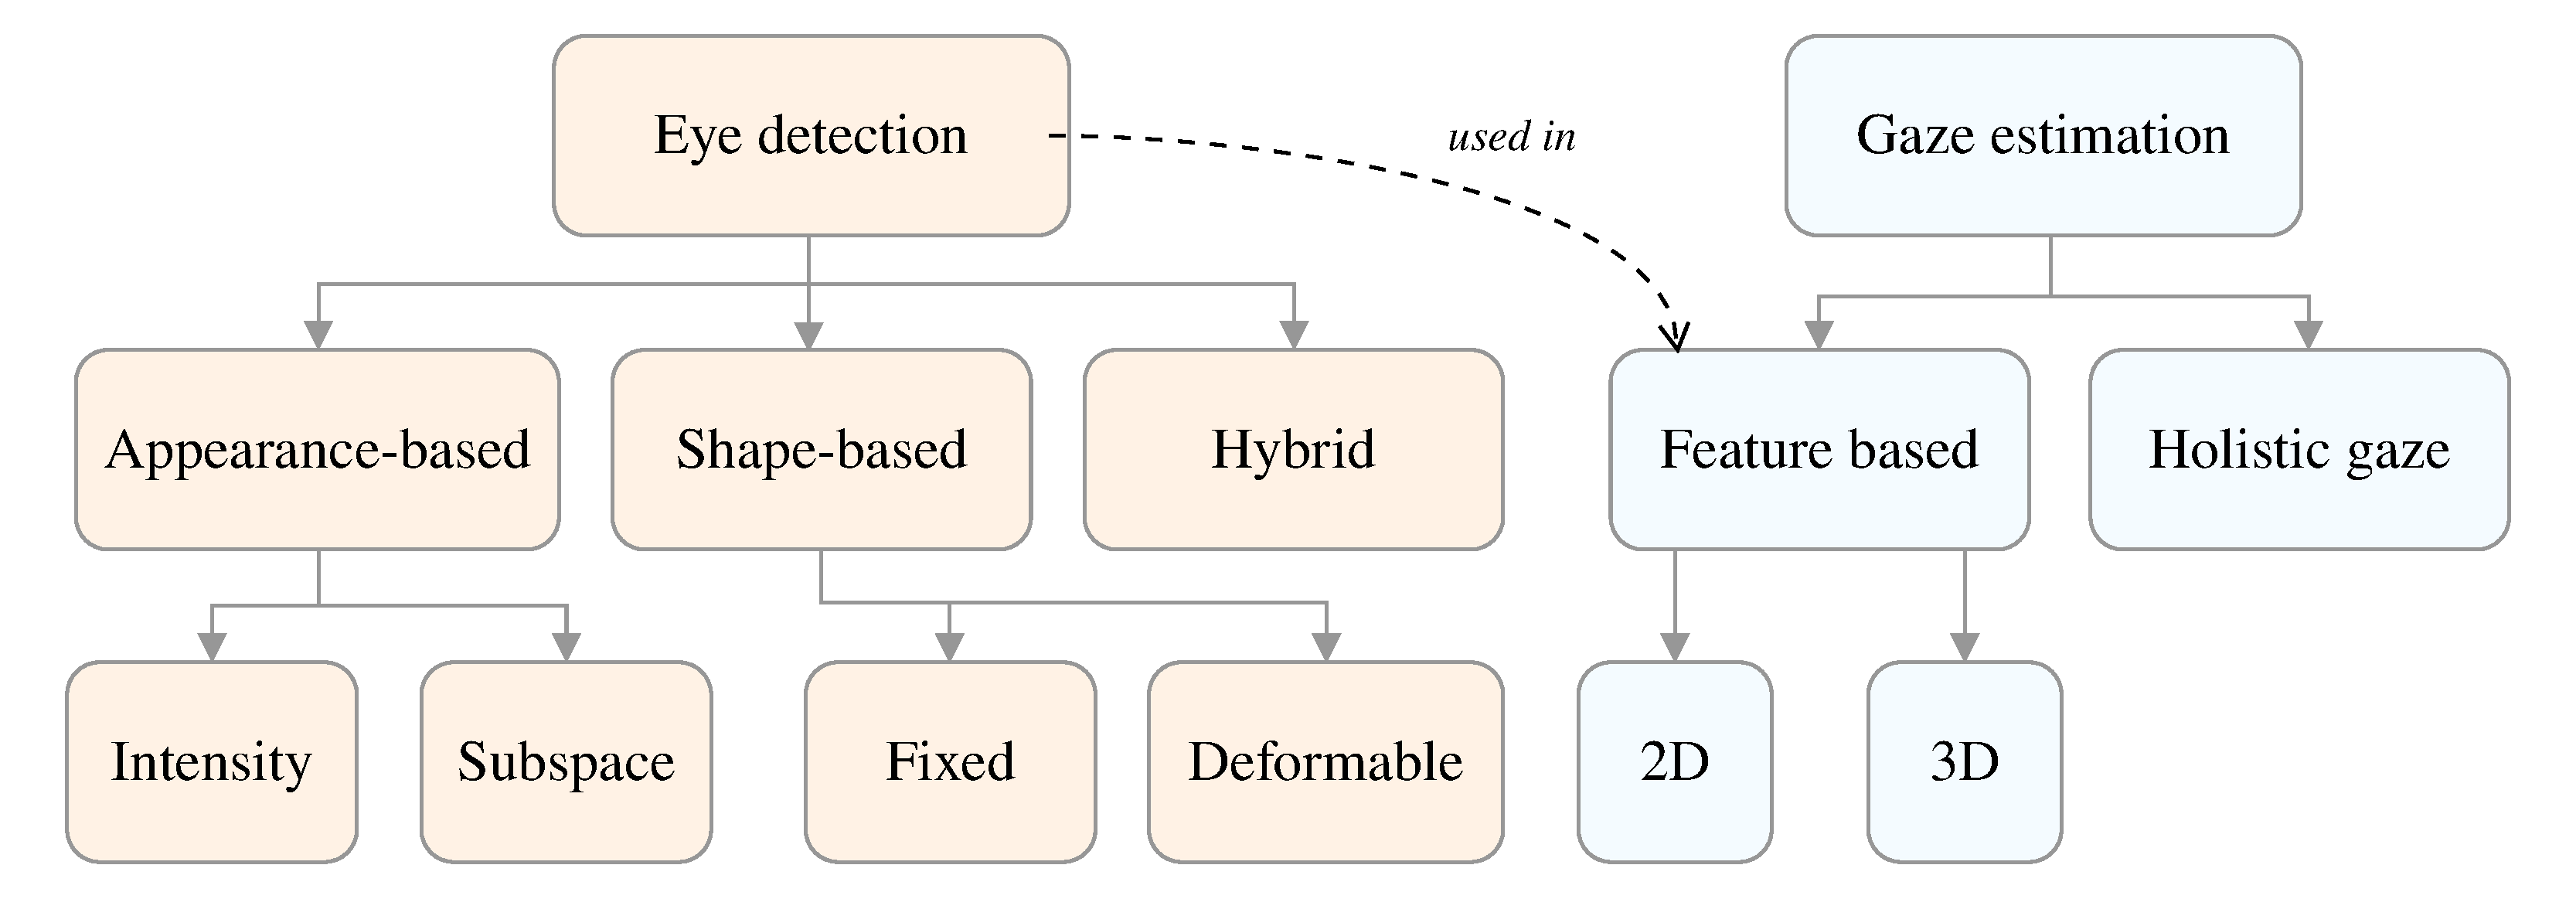
\includegraphics[width=1\textwidth]{figures/model/taxonomy}
	\caption{Eye tracking taxonomy.}\label{fig:taxonomy}
\end{figure}
All eye-tracking systems are composed of some common elements. \cref{fig:taxonomy} shows a possible component schematic of such a generalised system. At the most abstract level - an eye tracker works by capturing images of one or both of the subject's eyes and uses a number of different techniques to track the eyes themselves and to predict gaze. Because the use cases vary widely, a number of important classifications exist based on the hardware setup as well as the analysis methods employed.

The capturing setup is primarily determined by the relative mounting position of the eye-facing camera relative to the subject. In \gls{head-mounted} \gls{eye-tracking},  the eye-facing camera is fixed relative to the head of the subject and hence translational movements of the eye are kept to a minimum. The alternative is remote\todo{glossary} \gls{eye-tracking} where the camera is not fixed to the head and therefore allows more degrees of movement. Head-mounted eye-trackers may typically be augmented by a \gls{scene-camera} which points directly away from their head and can thus be used to determine what they are looking at a given point in time. \Gls{head-mounted} \gls{eye-tracker}s are often used when high-precision detection or gaze estimation is needed but comes at the cost of being less convenient to set up than a remote camera. Remote setups may provide high-precision eye-tracking if the head is fixed using a chin-rest or similar. The precision gained by fixing the relative position of eye and camera most stems mainly from the much higher utilisation of the image resolution as the eye can fill the entire image. Eye-tracking precision is generally affected by the environment, which is why controlled environments are generally preferred if possible. In many cases however, such as attention analysis, the environment cannot be controlled .... \todo{Example images and hardware setups!}

Eye-tracking systems cover a large range of use cases that require the detection of different properties. \Gls{gaze} is the most widely used end-product which may itself be used in secondary analyses of other personal properties (SECTION EYEINFO). Other important products include the iris and sclera textures which may be used for personal identification (REF) and the size of the pupil as it changes in response to external stimuli (REF). \Gls{gaze} is also typically used for eye movement analysis which produces an event-based overview of what kind of movements occur at given points in time (REFS). The different end-products have different requirements, but they all share the fundamental concept of being properties of interest that should be extracted from the source eye images. This generalisation idea is built upon in later sections (SECREF) to provide a theoretical model for eye-tracking that is useful for analysing privacy.... \todo{decide whether things should be added}

The property detection methods, of which there may be many or few in a given eye-tracking system, are typically classified as either appearance-based or feature-based. However, because of how modern systems including convolutional neural network (CNN) based ones makes the line seem less clear-cut, I redefine the two classes as holistic and local approaches after the same terms used in (dan REF). Figure (REF) shows the classification scheme. Holistic approaches consider the eye in its entirety, either by methods such as template matching (REF), or machine learning models such as CNNs mapping images directly to gaze. Local approaches instead consider specific eye elements or image features which are then combined. 

Eye-trackers may mix these methods. For example, CNNs which are inherently appearance-based have been shown to be extremely accurate at predicting the pupil centre which is then used in a two-dimensional gaze estimation model whic

\todo{Continue!}

%appearance-based and feature-based methods. The former covers methods that use the source image appearance to predict an output property

%Appearance-based methods use the image appearance itself to determine some property, e.g. eye position. This can be done either by template matching (REF), filter responses, or, more widespread today, using neural networks (REFS). 

%Feature-based 
%Shape-based models cover methods that try to fit a prior eye shape model to a single or several features in the image. Feature-based approaches aim at detecting non-typical features such as corneal reflections of LED lights or eye corners.


%Gaze estimation models are generally divided into two-dimensional models, three-dimensional models, and appearance-based models. The former two use detected eye features for gaze estimation and are therefore often collectively referred to as feature-based methods (REF dan). This is not to be confused with the feature-based paradigm itself although the two are often used together.

%The image based methods, which are the sole focus in this thesis, are typically broken down into components as shown in (FIGREF). Generally, the steps of eye detection and gaze estimation are separate, but in the case of \emph{appearance-based} gaze estimation, the image is mapped directly to gaze and thus skips the detection step. This approach is dominated by deep neural networks (REFS) and is most prominent in settings 



%Depending on the approach used, eye detection and gaze estimation may be individual steps or combined. 

%Knowing where people are looking is useful both for studying human behaviour and providing interactive technologies. 

%Eye-tracking is a scientific field that cover many different disciplines from computer science and engineering to psychology and biology. These can be divided into the research in eye-tracking technology and research enabled by eye-tracking technology. This section focuses on the former. It gives a short introduction to the eye-tracking technologies available today, how they work, and where they are used.


\section{Privacy}\todo{Needs a lot of glue and rewriting of old material}
This section presents potentially sensitive information sources in eye-tracking systems. The first part focuses on sensitive information that is extracted directly from eye images and the second part focuses on information derived from gaze signals.


Privacy is informally understood as the ability to hide information relating to your person from others. In technical terms, privacy is typically understood as the protection of information by modifying it in a way that allows only access by those who are authorised to do so. The paradox here is that the information 

 linked with probability 

 understood as the probability of ...
 
 

%\begin{displayquote}
%No one shall be subjected to arbitrary interference with his privacy, family, home or correspondence, nor to attacks upon his honour and reputation. Everyone has the right to the protection of the law against such interference or attacks.	
%\end{displayquote}


\begin{definition}[Sensitive information] 
	is any information related to a person that can be differentiated from others. This definition is a paraphrasing of the GDPR-equivalent.
\end{definition}

\begin{definition}[Privacy]
	in the context of information systems is a measure of how difficult it is to extract some property which should be hidden. 
\end{definition}


Sensitive information is thus the properties that cannot be shared freely without ethical and legal implications. Privacy is a measure of how secure a given method is at preventing that the information is shared. Encryption methods typically provide probabilistic guarantees that are so extreme that they are considered unbreakable (REF). These are however not useful in all situations.

Eye tracking data is created for the purpose of being consumed by some other process, whether it is in \acrshort{hci} or psychology. Encrypting the data, however, does not necessarily ensure protection for the user. In cases where the data is meant to be shared publicly, this is obvious by its definition. In other products, encryption only protects potential outside attackers from gaining access to the information. The producer of a given product still has the ability to use the information for various purposes and even if they don't intend to, the very presence of the information has legal implications in many areas of the world.


As mentioned briefly in (SECREF 2.1), eyes reveal many things about us. 

In this section, I outline known methods to exploit eye-tracking data for personal identification. Although iris-recognition is the most prominent method known today, other intriguing methods for identifying people based just on data on their eyes appearance or movements exist. Additionally, methods for determining a location or retrieving other personal information from e.g. scene cameras will also be presented.

\subsection{Personal identification}
Personal identification is one of the most serious privacy issues in eye-tracking since it makes it possible to link identity with other sensitive pieces of information. Using iris recognition specifically, it is possible to identity people with extremely high precision (REF). 

\subsubsection{Iris recognition}
The iris pattern in human eyes is unique and highly variable, even among twins and the left/right eye of a specific human being. It is also impossible to modify without risking damage to the eye \parencite{DAUGMAN_IRIS_ORIG}. Combined with the fact that fake eyes or lenses can be easily detected by utilising the contracting reflex of the pupil \parencite{DAUGMAN_IRIS_ORIG}, it makes the iris pattern an extremely valuable biometric. Genetics determine only the large-scale factors of the iris such as color, while the rest of its structure depends largely on initial conditions in the developing embryo \cite{kronfeldCHAPTERGrossAnatomy1962}, thus making it highly unique. 

A plethora of iris recognition methods exist. The most widely used and well-documented method is developed by John Daugman and uses Gabor wavelets \cite{daugmanHighConfidenceVisual1993} to produce a 2048-bit code for a given iris image. Identification is commenced by performing a test of statistical independence on the hamming distance between the two codes. If it fails the test, the codes are said to be a match. \autoref{fig:hamming-dist} shows the distributions of the hamming distance for similar and different irises. By adjusting the threshold for acceptance, Daugman achieves false-positive rates of as low as $10^{-13}$. This method will be used in a simplified form for the prototype presented in \autoref{sec:iris-recognition}.



In general, iris recognition methods can be categorised by their feature extraction methods. The process always starts with iris detection, segmentation, and conversion to \emph{pseudo-polar} coordinates resulting in images such as \autoref{fig:iris-code}. This raw image input is then used for extracting features that exhibit useful properties for iris identification such as lighting invariance and robustness to angle and focus.


The most common feature extraction methods are by far wavelet filter transforms \parencite{daugman2007new, ma2002iris, ma2004efficient, poursaberi2006iris, rydgren2004iris, zhu2000biometric} followed by frequency analysis techniques such as the discrete cosine transform\cite{iris-dct, monroDCTBasedIrisRecognition2007} and, more recently, deep learning based feature extractors\cite{gangwarDeepIrisNetDeepIris2016, nguyenIrisRecognitionOfftheShelf2018}.

\subsubsection{Sclera recognition}
Another measurable physical eye feature is the blood vessels in the sclera. As stated by several studies \cite{dasScleraRecognitionSurvey2013, zhouNewHumanIdentification2012}, the blood-vessels are stable over time, although the amount of literature supporting this is relatively sparse compared to iris patterns.

Methods for recognition include simple edge-filter responses with support-vector machines for classification \cite{dasNewEfficientAdaptive2014} as well as more complex processes involving the detection of individual blood vessel line segments \cite{zhouNewHumanIdentification2012}. Both methods achieve false positive rates around $10^{-2}$ for genuine acceptance rates around $80\%$.

\subsubsection{Identification based on eye movements}
Both iris and sclera recognition require relatively sharp and large eye images to be feasible. Eye movements, however, is exactly the goal of most eye-tracking systems. Of special concern is remote systems such as \cite{zhangMPIIGazeRealWorldDataset2017} that are specifically designed to track gaze based on remote camera sources such as webcams. Despite this ease of access, identification based eye movement currently suffers from some of the same problems as facial recognition, namely a much higher uncertainty and susceptibility to the recording circumstances.

Eye movement consists of multiple modes of operation. During a \emph{fixation}, the eye is relatively, but not completely, still as it focuses on a specific point. \emph{Saccades} are quick movements of the eyes and are split into macro-saccades and micro-saccades. The former describes the regular fast movement between fixations while the latter describes involuntary adjustments occurring even during fixation. \emph{Vergence shifts} describe movements to adjust binocular vision to perspective effects. Finally, \emph{smooth-persuit} movements describe the eye's ability to smoothly follow a moving object \cite{duchowskiBreadthfirstSurveyEyetracking2002}.

Identification is typically performed by comparing recorded eye movement features and testing for a statistically significant difference for rejection. Ioannis Rigas, George Economou, and Spiros Fotopoulos \cite{rigasBiometricIdentificationBased2012} present a method designed around clustering eye fixations and treating them as graphs to determine similarity. The fixations are gathered by presenting subjects with several images multiple times with the same images shown to all subjects. Other methods include feature extraction from reading scan-paths \cite{hollandBiometricIdentificationEye2011, bednarikEyeMovementsBiometric2005} and the use of Gabor filter responses to create features from scan-paths to be classified by a support vector machine\cite{liBiometricRecognitionTexture2018}. The methods all achieve much higher false acceptance rates than iris and sclera recognition methods however and it remains to be seen how effective they are in practice.

\subsection{Attribute estimation}















